%%%%%%%%%%%%%%%%%%%%% chapter.tex %%%%%%%%%%%%%%%%%%%%%%%%%%%%%%%%%
%
% sample chapter
%
% Use this file as a template for your own input.
%
%%%%%%%%%%%%%%%%%%%%%%%% Springer-Verlag %%%%%%%%%%%%%%%%%%%%%%%%%%

\chapter{Support Vector Machine}

Riprendiamo il problema della classificazione, abbiamo cercato in tutti i modi di affrontarlo. Quindi abbiamo analizzato il caso in cui i campioni sono etichettati, il caso in cui invece i campioni non sono etichettati. In entrambi i casi abbiamo supposto un sottocaso in cui abbiamo una forma parametrica nota di cui stimiamo soltanto i parametri ed un sottocaso invece in cui non era conosciuta neanche la forma e quindi andava stimata (caso non parametrico). In qualsiasi caso però ci siamo accorti che è più facile classificare se la superficie di decisione è una retta o un iperpiano, un esempio è il classificatore lineare che è stato utilizzato all'inizio, però è ovvio che per utilizzare il classificatore lineare i dati dovrebbero godere di certe caratteristiche essenziali. Nel caso in cui i dati non sono linearmente separibili allora abbiamo visto il classificatore quadratico e nel caso ancora più generale con i metodi non parametrici possiamo addirittura inseguire il contorno utilizzando una superficie di decisione polinomiale di grado $n$, dove però è difficile determinare i parametri del polinomio. L'ottimo però sarebbe quello di trasformare i dati in modo tale da utilizzare una superficie di decisione lineare, quindi che sia una retta o un iperpiano.  Alla base di questo ragionamento c'è una teroria che oltre alle support vector machine ha dato origine anche ad i metodi kernel, di cui l'SVM è un caso speciale. Distinguiamo in questo caso speciale il caso in cui i dati sono già linearmente separabili ed i dati che non sono linearmente separabili. Adesso verrà visto come progettare un SVM per i dati linearmente separabili, per poi estenderlo a dataset non linearmente separabili utilizzando la funzione kernel come trucco. \\

\section{Caso linearmente separabile}
\noindent La differenza tra un dataset linearmente separabile ed un dataset non linearmente separabile è nota..... L'SVM ha una particolarità, non è un classificatore qualsiasi ma è un classificatore binario, cioè non si applica a più classi ma si applica a due classi. Però può essere esteso al caso multiclasse. Come al solito i pattern sono vettori di caratteristiche (spazio delle features). L'idea è che se io riuscissi a proiettare i pattern in un altro spazio di dimensioni maggiori rispetto allo spazio di origine ma con la particolarità che nel nuovo spazio i pattern godono della proprietà rispetto agli originali di essere linearmente separabili, se accade questo allora il problema si risolve semplicemente applicando un classificatore lineare.\\

\noindent Perchè l'acronimo SVM? SVM sta per Support Vector Machine ovvero Macchina di classificazione di vettori oppure macchina a vettori di supporto. Sono vettori $n$ dimensionali, le dimensioni sono relative alle $n$ caratteristiche. Invece il termine \emph{vettori di supporto} allude al fatto che alcuni di questi pattern hanno un ruolo importante nell'identificazione della retta o dell'iperpiano, cioè della superficie di decisione che da ora in poi verrà chiamato margine massimo.\\

\noindent Dato un training set $\mathcal{D}$, stiamo nel caso supervisionato e di conseguenza per ogni pattern conosciamo la classe di appartenenza, ciascun osservazione è composta da un coppia di un vettore $\mathbf{x}_i$ e da una verità $y_i$ che può essere $+1$ o $-1$. Adesso vogliamo che il classificatore si addestri su un training set per poi saper classificare un test set (pattern che non ha mai visto). La capacità di classificare un test set è detta capacità di generalizzazione. L'obiettivo è quello di ottenere una buona percentuale di classificazione sul test set. Per ottenere questo bisogna trovare un giusto equilibrio tra la capacità della macchina di apprendere un qualsiasi training set e la classificazione ottenuta su un test set. Se per esempio si ottiene il $100\%$ di classificazione su un training set significa cha la macchina di apprendimento ha funzionato correttamente sull'insieme di dati per i quali è stata addestrata, di maggiore interesse è invece il risultato ottenuto sulla classificazione di un test set, nel caso in cui le percentuali sono basse allora è successo che il classificatore ha appreso esclusivamente il training set e non ha capito quel'è la funzione che sta dietro tutti di i dati. Es.: se ho un dataset su 1000 dati e la macchina si specializza solo su 100 dati allora significa che non sarà in grado di classificare i restanti dati, quindi non ha capito la funzione che generalizza la classificazione. Quindi si vuole riuscire a dedurre (fare un inferenza) dai 100 dati la funzione che sta dietro tutti 1000 dati, e non è una cosa banale. Questa capacità viene perfezionata grazie all'uso del \emph{validation set} che è una tecnica per migliorare la generalizzazione. L'idea è quella di dividere il dataset in tre parti, un training set, un validation set ed un test set. La macchina viene addestrata sul training set e la validazione viene effetuta  sul validation set, quindi questa procedura va avanti finché non sono state raggiunte buone percentuali di classificazione sul validation set. Riassumendo i passi sono quelli di addestrare la macchina sul training set, misurare le percentuali di classificazione dell'addestramento sul validation set, ci si ferma quando la percentuale ottenuta sul validation set è soddisfacente, dopo lo si applica sul test set per avere la capacità di generalizzazione. In questo modo la macchina apprende anche a generalizzare. \\

\noindent L'obiettivo principale è quello di trovare la retta che suddivide i dati che abbiamo detto essere linearmente separabili
\begin{equation}
\mathbf{x}_i \mathbf{w} + b = 0
\end{equation}
Un insieme di dati è linearmente separabile, quando è possibile trovare una coppia $(w,b)$ tale che
\begin{gather}\label{166}
\mathbf{x}_i \mathbf{w} + b \geq +1	\ \ \text{per} \ \ y_i=+1\\
\mathbf{x}_i \mathbf{w} + b \leq -1	\ \ \text{per} \ \ y_i=-1
\end{gather}
L'obiettivo è quello di suddividere lo spazio in due parti, una per la quale ai pattern viene data risposta 1 mentre per l'altra parte viene data risposta -1. Solo in questo caso possiamo dire che il dataset è linearmente separabile, quindi c'è una retta che li separa. SVM trova proprio questa retta, non una semplice retta ma una retta particolare, trova la retta a margine massimo. Introduciamo $d+$ e $d-$ come la minima distanza  tra il piano separatore ottimo ed il punto positivo e negativo più vicino, fra le due classi è possibile inclinare la retta in molti modi ma si tende a scegliere una retta che sta in mezzo per evitare l'errore. Si capisce subito che dalle disequazioni \ref{166} la funzione che assume valore $+1$ o $-1$ è la funzione segno. Come si può trovare ls retta ottima? Sappiamo che l'equazione della retta è del tipo $xy + b = 0$ se invece $\mathbf{x}$ è un vettore $n$-dimensionale allora $\mathbf{x}\mathbf{w} + b = 0$ è l'equazione dell'iperpiano. Sicuramente sappiamo che $\mathbf{w}$ è il vettore dei pesi che si trova perpendicolare al piano o alla retta, $b$ è l'intercetta. Inoltre sappiamo anche che $\frac{\abs{b}}{\norma{\mathbf{w}}}$ è la distanza ortogonale del piano dall'origine. Definiamo margine di un piano separatore o di una retta separatrice il valore $d+ \ + \ d-$ cioè la somma della distanze che intercorre tra il punto punto più vicino di una classe e la retta o piano ed il punto più vicino dell'altra classe alla retta o piano(Fig \ref{svm}).
\begin{figure}
\centering
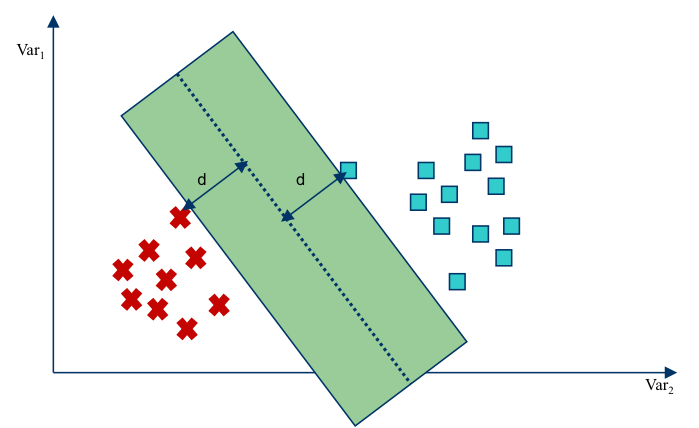
\includegraphics[scale=1]{img/svm.png}
\caption{Margine massimo}
\label{svm}
\end{figure}
La somma delle due distanze minime è chiamato margine. Dato che la funzione segno assume $+1$ per valori positivi e $-1$ per valori negativi, come detto in precedenza la funzione che soggiace è $f(x)=segno(\mathbf{x}\mathbf{w} + b)$, allora argomento e valore della funzione sono concordi in segno, quindi possiamo scrivere il tutto come
\begin{equation}
y_i(\mathbf{x}\mathbf{w} + b) \geq 1
\end{equation}
Come trovare la retta ottimale? Supponiamo i punti per cui è verificata l'equazione \ref{166}, questi punti giacciono sull'iperpiano $\mathbf{x}\mathbf{w} +b = 1$ con normale $\mathbf{w}$ e distanza dall'origine $\frac{\abs{1-b}}{\norma{\mathbf{w}}}$ che chiamiamo H1. Analogamente i punti che soddisfano l'uguaglianza della seconda equazione si trovano sull'iperpiano H2: $\mathbf{x}\mathbf{w} + b = -1$ con la stessa normale $\mathbf{w}$ e distanza dall'origine $\frac{\abs{-1-b}}{\norma{\mathbf{w}}}$. Questi due luoghi di punti nel caso bidimensionale sono rette. H1 e H2, avendo la stessa normale, sono paralleli e osserviamo che nessun vettore di training cade tra essi. I vettori di supporto sono quei pattern che sono più vicini alle rette ottime per la classe e sono di supporto all'iperpiano. Adesso dobbiamo trovare l'iperpiano ottimale. Sommando le due distanze dall'origine abbiamo $\frac{2}{\norma{\mathbf{w}}}$, ci accorgiamo che questo è il margine che ottengo nel caso generale. Allora possiamo dire che il margine massimo è $\frac{2}{\norma{\mathbf{w}}}$ e allora la massimizzazione del margine dipende da $\norma{\mathbf{w}}$, quindi se minimizzo $\norma{\mathbf{w}}$ allora massimizzo $\frac{2}{\norma{\mathbf{w}}}$. Quindi massimizzare il margine equivale a minimizzare $\norma{\mathbf{w}}$. In particolare per risolvere minimizzo $\frac{1}{2} \norma{\mathbf{w}}$ soggetto però ad un vincolo, cioè che i segni della funzione siano concordi quindi $y_i(\mathbf{x}\mathbf{w} + b) \geq 1$. Questo è il problema da risolvere. Ci appelliamo alla teoria della regolarizzazione utilizzando il moltiplicatore di lagrange.\\
 
\noindent Cosa si fa? adesso la funzione diventa $\frac{1}{2} \norma{w}^2$. Minimizzare $w$ equivale a massimizzare $y_i(xw + b) - 1$ o equivalentemente a minimizzare $-y_i(xw + b - 1)$, ricapitolando la funzione da minimizzare è $\frac{1}{2} \norma{w}^2$ con il vincolo visto precedentemente, quindi con il meno davanti non faccio altro che minimizzare $-y_i(xw + b - 1)$, così la funzione diventa 
\begin{equation}
L(w,b,\Lambda) = \frac{1}{2} - \sum_{i=1}^l \lambda_i \left[ y_i (xw + b) - 1\right]
\end{equation}
utilizziamo la sommatoria perché lo eseguiamo per ogni pattern, quindi devo aggiungere tanti vincoli quante sono queste le situazioni, ognuno avrà un proprio moltiplicatore di lagrange che viene indicato con $\lambda_i$. Il moltiplicatore sta a indicare un peso che voglio dare al vincolo nella funzione da minimizzare. Ci troviamo di fronte al caso di una minimizzazione di un funzionale, i parametri $w$ si trovano semplicemente facendo il gradiente o la derivata parziale rispetto a $w$ e ponendola uguale a zero. Ricordiamo che c'è anche il parametro $b$, quindi faccio la derivata anche rispetto a $b$, dove il $b$ è il bias. 
Quindi la derivata parziale rispetto a $w$ è
\begin{equation}
\frac{\partial L(w,b,\Lambda)}{\partial w} = w - \sum_{i=1}^l \lambda_i y_i x
\end{equation}
mentre rispetto a $b$ è
\begin{equation}
\frac{\partial L(w,b,\Lambda)}{\partial b} = \sum_{i=1}^l \lambda_i y_i
\end{equation}
ponendo la derivata parziale rispetto a $w$ uguale a zero otteniamo
\begin{gather}
w - \sum_{i=1}^l \lambda_i y_i x = 0\\
w^* = \sum_{i=1}^l \lambda_i^* y_i x 
\end{gather}
I parametri che conosco sono $x_i$ ed $x_j$ ma conosco anche $y_i$ ed $y_j$ dato che stiamo parlando di un apprendimento supervisionato, quindi non conoscono soltanto i moltiplicatori di lagrange, effettuando alcune sostituzione posso far diventare la funzione soltanto funzione dei moltiplicatori
\begin{equation}\label{174}
F(\Lambda) = \sum_{i=1}^l \lambda_i - \frac{1}{2} \norma{w}^2 = \sum_{i=1}^l \lambda_i - \frac{1}{2} \sum_{i,j=1}^l \lambda_i \lambda_j y_i y_j x_i x_j
\end{equation}
Abbiamo visto che il valore ottimale $w^*$ è semplicemente la sommatoria del prodotto $x_i y_i$ ognuno moltiplicato per il proprio moltiplicatore di lagrange. Quindi il problema adesso si riduce a trovare i moltiplicatori di lagrange ottimali ottenuti risolvendo la \ref{174}, in particolare massimizzando quella funzione. Quindi dal problema di trovare i parametri $w$ per i quali il margine è massimo mi ritrovo a massimizzare un altro funzionale che dipende esclusivamente dai moltiplicatori di lagrange. In conclusione trovati i moltiplicatori li vado a sostituire per trovare i parametri $w$. Il valore ottimale $w^*$ è quello che poi va sostituito nell'equazione della retta per ottenere la retta separatrice. Il classificatore è dato da 
\begin{equation}
class(x_k) = \text{sign} \left( \sum_{i=1}^m \lambda_i y_i x_i \cdot x_k + b\right)
\end{equation}

\section{Caso non linearmente separabile}
Questo stesso problema si può applicare anche a dati che non sono linearmente separabili (fig \ref{svm2}).
\begin{figure}
\centering
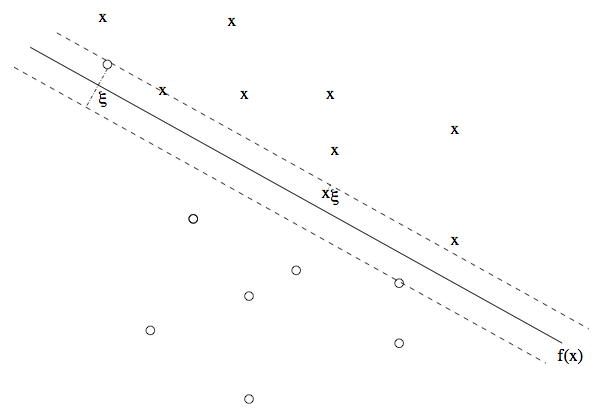
\includegraphics[scale=0.5]{img/svm2.png}
\caption{Caso non linearmente separabile}
\label{svm2}
\end{figure}
Naturalmente non ci attendiamo una separazione netta tra le classi ma ovviamente cerchiamo il minimo errore, per fare questo si utilizza una tecnica di ottimizzazione, una tecnica che usa le variabili fittizie o variabili slack, queste variabili non negative le indichiamo con
\begin{equation}
\xi = (\xi_1, \dots, \xi_l)
\end{equation}
queste variabili permettono di modellare il fatto che alcuni vincoli di disugualianza possono essere violati.
Alla fine non ho più la separazione netta tra i pattern che hanno il target -1 e quelli che hanno 1, ma ho una forma di indecisione, quindi per ogni punto ho un indecisione relativa alla sua collocazione. Questa indecisione è $1-\xi_i$, che può diventare un valore in modo tale da alterare l'assegnazione di $x_i$.Data questa imposizione il tutto viene modificato nel seguente modo
\begin{equation}
y_i(\mathbf{x}\mathbf{w} + b) \geq 1 - \xi_i
\end{equation}
il valore di $\xi_i$ è 0 quando la locazione è corretta, è maggiore di uno quando la locazione non è corretta ed è compreso tra zero ed uno quando ci si trova di fronte ad una situazione di indecisione.\\

\noindent A questo punto sorge la domanda. Ma è possibile portare un insieme di dati non linearmente separabili in un insieme di dati linearmente separabili? L'obiettivo sarebbe quello di prendere i dati, riuscire a proiettarli in uno spazio diverso in modo tale che però i dati risultano linearmente separabili. Qual'e trasformazione ci consente di fare ciò? una funzione $\Phi$. Possiamo scegliere la $\Phi$ come vogliamo.\\

\noindent L'identificazione dell'iperpiano di separazione ottimo è molto più difficile quando si usano queste variabili slack, poiché per un classificatore ottimo bisogna trovare un compromesso tra due condizioni opposte. Da un lato un buon classificatore SVM corrisponde ad un iperpiano (w,b) con il massimo margine possibile per garantire una buona classificazione, il si traduce in minimizzare $\frac{\norma{w}^2}{2}$. Dall'altro lato l'iperpiano ottimo dovrebbe minimizzare il numero degli errori e dei pattern mal classificati, il che si traduce in minimizzare il numero delle variabili slack positive e allo stesso tempo minimizzare il valore di ogni variabile. La seconda è in contraddizione con la prima in quanto tende a far decrescere il margine massimo. Un semplice modo per combinare queste due condizioni è quello di assegnare una penalità per ogni errore di classificazione. Quindi la funzione viene da minimizzare è
\begin{equation}
\frac{\norma{w}^2}{2} + C\left( \sum_{i=1}^m \xi_i \right)^k
\end{equation}
con i vincoli 
\begin{gather}
y_i (w \cdot x_i + b) \geq +1 - \xi_i \\
\xi_i \geq 0
\end{gather}
per ogni $i=1, \dots, m$. Dove $C$ è un parametro che può essere regolato dall'utente. Quando $C$ è grande viene assegnata un alta penalità dovuta agli errori, un piccolo $C$ massimizza il margine e di conseguenza è meno sensibile agli errori. \\

\noindent Anche in questo caso per risolvere il problema viene seguito l'approccio basato sui moltiplicatori di Lagrange. Vengono definiti i moltiplicatori di Lagrange $\Lambda =(\lambda_1, \lambda_2, \dots, \lambda_m)$ per ogni vicolo $y_i (w \cdot x_i + b) \geq +1 - \xi_i$, poi vengono definiti i moltiplicatori $M= (\mu_1, \mu_2, \dots, \mu_m )$ per ogni vincolo $\xi_i \geq 0$, la funzione per questo problema è
\begin{equation}
L_p = (w,b,\Lambda, M)  =  \frac{\norma{w}^2}{2} + C \sum_{i=1}^m \xi_i - \sum_{i=1}^m \lambda_i \left[ y_i (xw + b) - 1 + \xi_i \right] - \sum_{i=1}^m \mu_i \xi_i
\end{equation}
Anche in questo caso i parametri $w$ si trovano semplicemente facendo il gradiente o la derivata parziale rispetto a $w$ e ponendola uguale a zero. Viene effettuata la derivata parziale rispetto a tutti i parametri che entrano in gioco. Il risultato è
\begin{equation}
w =  \sum_{i=1}^l \lambda_i y_i x 
\end{equation}
La soluzione al problema è identica a quella del caso separabile tranne per il vincolo sui moltiplicatori che adesso sono limitati superiormente da $C$. 

\section{Support Vector Machine non lineari}
Nelle precedenti sezioni, è stato introdotto il classificatore SVM il quale usa pattern di training per generare un piano di separazione ottimo. Tali classificatori non sono adeguati per casi in cui esiste una relazione complessa tra i parametri di input e le classi dei pattern. \\

\noindent La superfice di separazione potrebbe essere non lineare in molti problemi di classificazione, la le SVM possono essere estese per gestire superfici di separazione non lineare usando una funzione $\Phi(x)$. L'idea è quella di mappare lo spazio delle dimensioni di input in uno spazio a più alte dimensioni con la caratteristica che in questo nuovo spazio si può eseguire una separazione lineare. Ci sono alcuni dataset per i quali neanche l'uso di variabili slack fornisce una soluzione al problema. La funzione non lineare $\Phi$ trasforma lo spazio delle dimensioni mappandole in uno spazio a più alte dimensioni ove però è possibile separare i dai linearmente. Ottenuto ciò basta eseguire un semplice SVM per ottenere la classificazione. L'unica difficoltà sta nell'identificare per un particolare dataset, il corretto insieme di funzioni non lineari che potrebbero eseguire questo mapping.\\

\noindent Consideriamo un training set $T$ di $m$ pattern e la loro etichettatura,\\
 $T=\{ (x_1, y_1), (x_2, y_2), \dots, (x_m, y_m) \}$, dove $x$ è un pattern ad $n$ dimensioni $x  = (x_1, x_2, \dots, x_n)$. Definire l'insieme delle funzioni $\Phi_1, \Phi_2, \dots, \Phi_b $. Ogni pattern è mappato in $\Phi(x)$
\begin{equation}
x = \Phi(x)
\end{equation}
Dopo aver mappato tutti i pattern del training set otteniamo un insieme di punti proiettati in un spazio più grande. Il classificatore diventa
\begin{equation}
class(x_k) = \text{sign} \left( \sum_{i=1}^m \lambda_i y_i \Phi(x_i) \cdot \Phi(x_k) + b\right)
\end{equation}
quindi è necessario calcolare il prodotto $\Phi(x_i) \cdot \Phi(x_k)$ per tutti i pattern. Per ovviare a questo problema si può introdurre una funzione kernel che restituisce il prodotto delle immagini dei suoi due argomenti $K(x_i,x_j) = \Phi(x_i) \cdot \Phi(x_k)$ e quindi è possibile evitare di eseguire il prodotto esplicito tra le immagini di due argomenti. Una funzione kernel è una funzione che ritorna il valore del prodotto interno fra le immagini di due argomenti. A questo punto è possibile inserire la funzione kernel all'interno dell'algoritmo ed ignorare la forma esplicita di $\Phi$. Possono essere utilizzati vari tipi di kernel: polinomiale, gaussiano, sigmoidale a doppia strato. 


%
